\documentclass[12pt]{beamer}
\usepackage[utf8]{inputenc}
\usepackage{polski}
\usepackage[english,polish]{babel}
\usepackage{graphicx}
\usepackage{hyperref}

\usetheme{Warsaw}
\usecolortheme{crane}
\author{Jakub Kuźma}
\title{Przykład zastosowania frameworku Ruby~on~Rails do stworzenia
  gry internetowej}
\setbeamercovered{transparent}

\begin{document}

\frame{\titlepage}

\begin{frame}
  \frametitle{,,Osadnicy z Catanu''}
  \begin{block}{Die Siedler von Catan}
    Wieloosobowa gra planszowa wymyślona przez Klausa Teubera, wydana
    po raz pierwszy w 1995.
  \end{block}
\end{frame}

\begin{frame}
  \frametitle{,,Osadnicy z Catanu'' - gra planszowa}
  \begin{figure}
    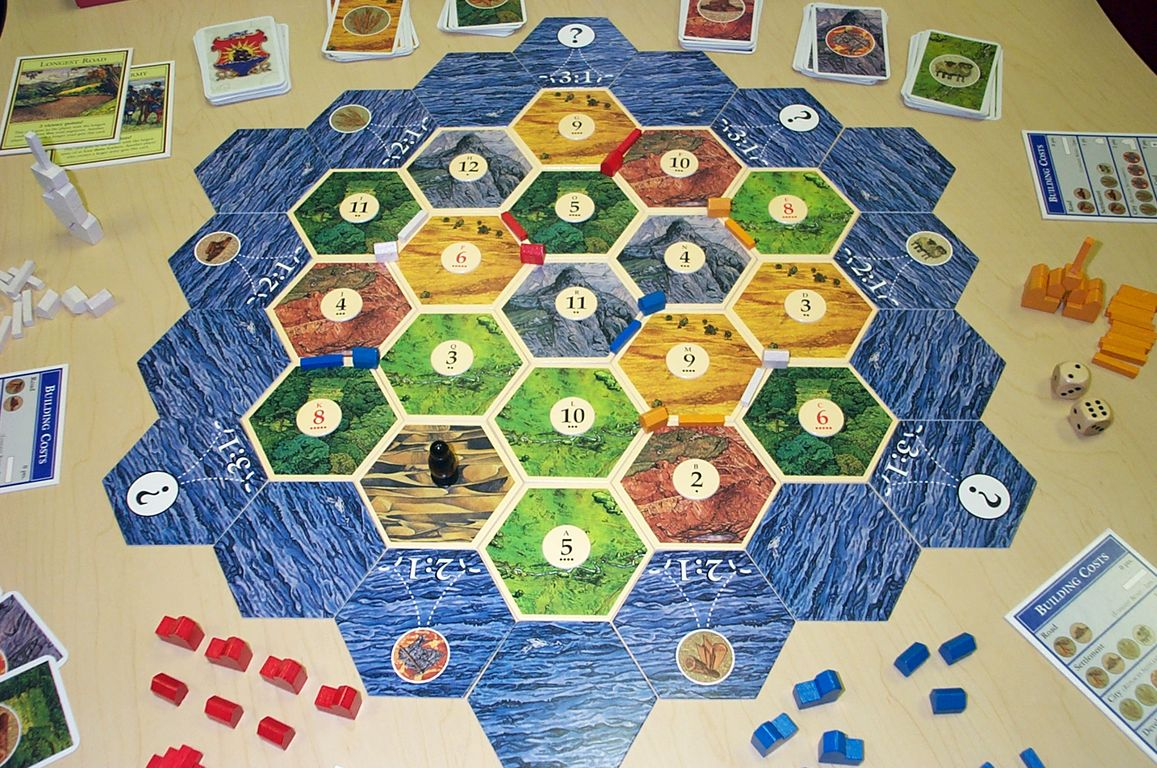
\includegraphics[width=\linewidth]{settlers.jpg}
  \end{figure}
\end{frame}

\begin{frame}
  \frametitle{Cel pracy}
  Aplikacja umożliwiająca prowadzenie wielu rozgrywek w grę ,,Osadnicy
  z Catanu'', wykorzystująca:
  \begin{itemize}
  \item Ruby on Rails - implementacja serwera
  \item JavaScript - implementacja klienta
  \item HTTP Pull, zgodnie z REST - komunikacja
  \item relacyjną bazę danych
  \end{itemize}
\end{frame}

\begin{frame}
  \frametitle{Dlaczego ,,Osadnicy z Catanu''?}
  \begin{itemize}
  \item stosunkowo niewiele implementacji
    % w porównaniu np. do szachów lub klasycznych gier karcianych
  \item rosnąca popularność
    % w Polsce od kilku lat rozgrywane są mistrzostwa, w tym roku w
    % Gliwicach
  \item prawie nieograniczone możliwości rozwoju
    % niezliczona ilość dodatków, modyfikacji (kilka oficjalnych i
    % wiele nieoficjalnych)
  \item dość duży stopień skomplikowania
    % nie chodzi o skomplikowanie rozgrywki (ciężko byłoby konkurować
    % z szachami czy brydżem) a ilość elementów, które należy
    % zaimplementować
  \end{itemize}
\end{frame}

\begin{frame}
  \frametitle{Dlaczego Ruby on Rails?}
  \begin{itemize}
  \item duża elastyczność
    % chodzi o pokazanie, że Railsy nadają się także do tworzenia
    % "nieszablonowych" aplikacji, w wielu miejscach wciąż można
    % usłyszeć, że jest to świetny framework do tworzenia blogów w 15
    % minut
  \item nowatorstwo rozwiązań
    % począwszy od 2004 roku (data wydania Railsów) co pewien czas
    % pojawiają się nowe frameworki, które w mniejszym lub większym
    % stopniu wzorują się na Railsach (Merb, Symfony, Grails, Lift)
  \end{itemize}
\end{frame}

\begin{frame}[fragile]
  \frametitle{Dlaczego REST?}
  \begin{itemize}
  \item prostota
  \item zmiana sposobu projektowania aplikacji
\begin{verbatim}
user.add_permission("write")
user.persmissions.create("write")
\end{verbatim}
  \item nie narzuca formatu wymiany danych
  \item umożliwia używanie wielu formatów jednocześnie
  \end{itemize}
\end{frame}

\begin{frame}
  \frametitle{Dlaczego JavaScript?}
  \begin{itemize}
  \item najpopularniejszy język programowania na świecie
    % interpreter tego języka znajduje się w niemal każdej
    % przeglądarce internetowej
  \item wysoka przenośność
    % aplikacja powinna działać również w urządzeniach przenośnych
  \item duża liczba potencjalnych odbiorców
    % brak dodatkowych wymagań typu Flash, Java, które nie są w pełni
    % dostępne na niektórych platformach
  \item chęć poznania języka
    % z bardziej prywatnych powodów - dość specyficzny język, znacznie
    % różniący się od ,,klasycznych'', warty poznania
  \end{itemize}
\end{frame}

\begin{frame}
  \frametitle{Dlaczego relacyjna baza danych?}
  \begin{itemize}
  \item domyślne rozwiązanie - najprostsze do wykorzystania
    % częścią frameworka jest biblioteka ActiveRecord, oferująca
    % tzw. mapowanie obiektowo relacyjne
  \item duża dostępność, niższa cena hostingu
    % mowa o początkowej fazie, przy większych aplikacjach ten element
    % jest zwykle wąskim gardłem, najkosztowniejszym i najtrudniejszym
    % w optymalizacji
  \end{itemize}
\end{frame}

\begin{frame}
  \frametitle{Dlaczego HTTP Pull?}
  \begin{itemize}
  \item działa we wszystkich współczesnych przeglądarkach
    % również w przeglądarkach mobilnych, czego nie można powiedzieć o
    % HTTP Push (przykład: GMail)
  \item nie wymaga dodatkowych serwerów - łatwiejszy hosting
    % do komunikacji wystarcza jeden serwer aplikacji
  \item opóźnienia nie mają większego wpływu na rozgrywkę
    % jeśli tylko pobieranie danych odbywa się w rozsądnie niskich
    % odstępach czasu
  \end{itemize}
\end{frame}

\begin{frame}
  \frametitle{Rezultaty}
  \begin{itemize}
  \item zaimplementowane zostały wszystkie elementy gry
    % takie jak handel, karty rozwoju
  \item wymaga jeszcze dużej ilości pracy
    % w szczególności część kliencka - uporządkowanie kodu,
    % zaprojektowanie grafiki i layoutu, przekracza to możliwości
    % jednej osoby
  \item możliwe jest logowanie użytkowników, tworzenie gier,
    dołączanie do nich i przeprowadzanie rozgrywek
    % czyli wszystkie najistotniejsze elementy, przy czym sama
    % rozgrywka nie należy do najprzyjemniejszych - należałoby
    % poprawić interfejs użytkownika
  \end{itemize}
\end{frame}

\begin{frame}
  \frametitle{Plansza do gry}
  \begin{figure}
    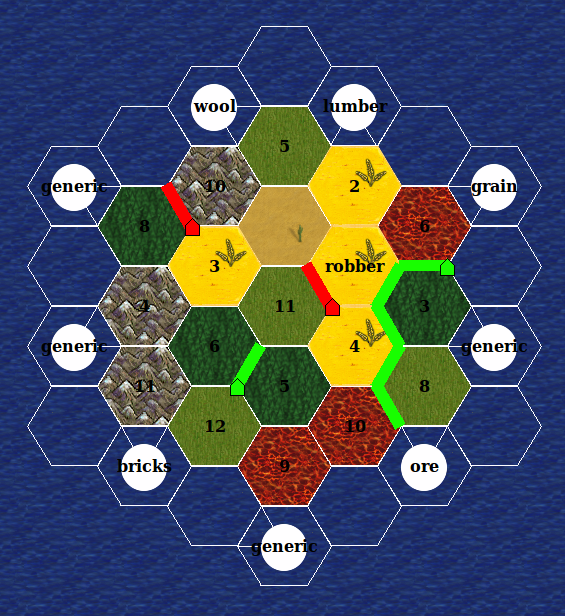
\includegraphics[width=0.6\linewidth]{board.png}
  \end{figure}
\end{frame}

\begin{frame}
  \frametitle{Wnioski}
  \begin{itemize}
  \item maszyny stanowe i biblioteka \emph{State Machine} znakomicie
    sprawdziły się w implementacji gry
  \item relacyjna baza danych była sporym utrudnieniem
    % gra musiała zostać rozdzielona na ponad 10 tabel, wymaga
    % częstych złączeń. Zdecydowanie lepiej byłoby użyć bazy danych
    % zorientowanej dokumentowo, takiej jak MongoDB
  \item tworzenie dużych aplikacji w języku JavaScript wymaga sporej
    wprawy (pomogła nieco zmiana biblioteki na \emph{YUI})
    % pół roku nie wystarcza, żeby opanować ten język w stopniu
    % umożliwiającym zaprojektowanie i zaimplementowanie tak dużej
    % aplikacji, w jQuery brakuje wielu przydatnych elementów
  \end{itemize}
\end{frame}


\end{document}
